\documentclass[12pt]{article}
\usepackage{fancyhdr,epsfig,graphics,tabularx,times}
\pagestyle{empty}
\topmargin=-0.75in
\oddsidemargin=-0.5in
\textwidth=7.5in
\textheight=10.25in
\parindent=0.0in
\parskip=10pt
\linespread{1.0}

\renewcommand{\labelenumi}{(\alph{enumi})}
\renewcommand{\thefigure}{\arabic{section}.\arabic{figure}}
\def\thesection{Problem \#\arabic{section}}

\begin{document}
{\bf BME154L - Spring 2012 - Exam \#2 Solutions}\hfill Name (Net ID):\underline{\hspace*{3.0in}}



\vspace*{0.5in}

\centerline{\LARGE BME354L (Palmeri)}
\vspace*{0.25in}
\centerline{\LARGE Spring 2013}
\vspace*{0.25in}
\centerline{\LARGE Exam \#2}
\vspace*{0.25in}

{\bf Instructions:} 
\begin{itemize}
\item Write your name at the top of each page.
\item {\bf Show all work (this is {\it critical} for partial credit!)}.
\item Remember to include units with all answers and label all plot axes.
\item Clearly delineate all answers.
\item Assume that all components are ideal unless otherwise stated.
%\item Assume that op amps rail at $\pm$ 12 V unless otherwise stated.
\item Please keep your answers brief for questions where I ask `why?'.
\end{itemize}

\vspace*{3in}

\emph{In keeping with the Duke Community Standard, I have neither given nor received aid in completion of this examination.}

\vspace*{0.5in}

Signature:\underline{\hspace*{3.0in}}


\clearpage

{\bf BME154L - Spring 2012 - Exam \#2 Solutions}\hfill Name (Net ID):\underline{\hspace*{3.0in}}



\section{[20 points]}

\begin{center}
\begin{tabular}{cc}
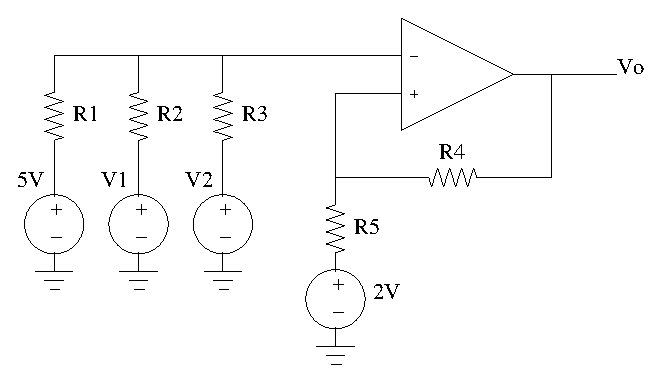
\includegraphics[width=0.6\linewidth]{sum_comparator.eps} &
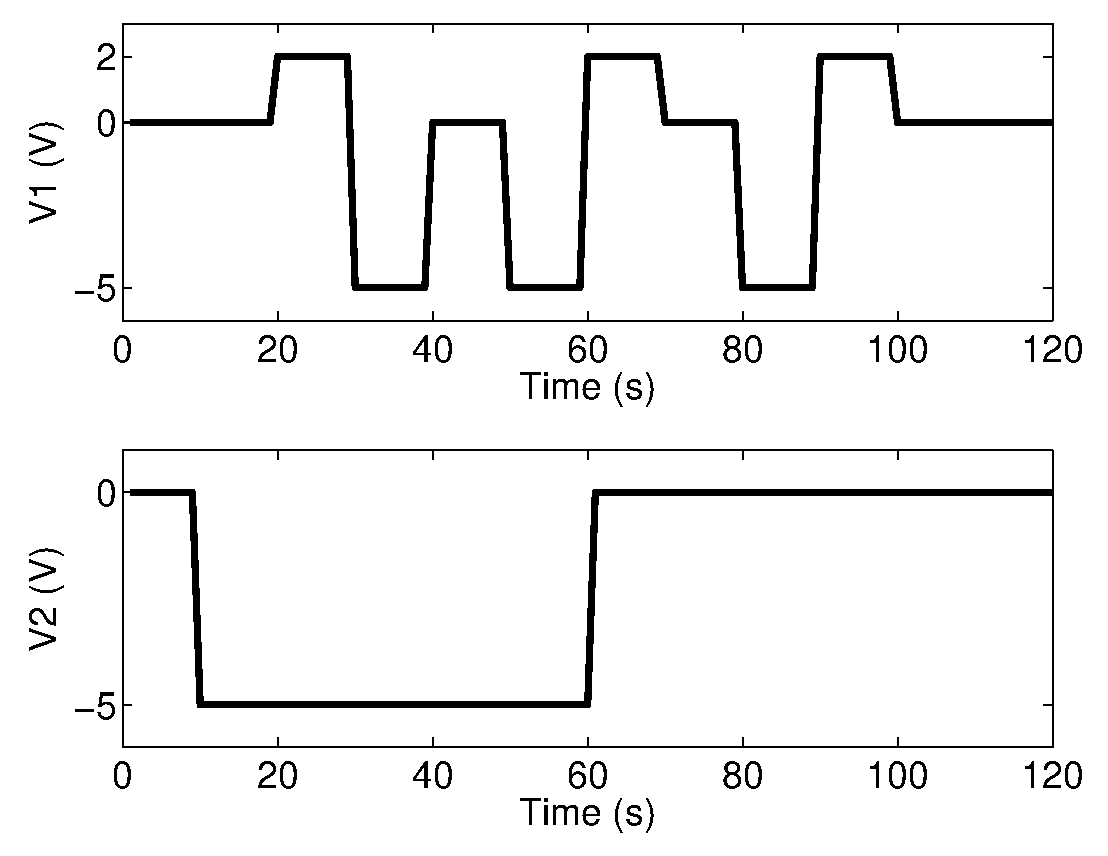
\includegraphics[width=0.4\linewidth]{sum_comparator_v1_v2.eps} \\
\end{tabular}
\end{center}

\begin{itemize}
\item $R_1$ = $R_2$ = $R_3$ = $R_4$ = $R_5$ = 1 k$\Omega$; $R_4$ = 9 k$\Omega$
\item Assume that the op amp rails at $\pm$ 12 V and $V_o$ = -12 V at t = 0
\end{itemize}

\begin{enumerate}
\item Given $V_1(t)$ and $V_2(t)$, sketch the voltage on the non-inverting input of
the op amp through time.
\item Sketch the output voltage, $V_o(t)$.
\end{enumerate}

\clearpage

{\bf BME154L - Spring 2012 - Exam \#2 Solutions}\hfill Name (Net ID):\underline{\hspace*{3.0in}}



\clearpage

{\bf BME154L - Spring 2012 - Exam \#2 Solutions}\hfill Name (Net ID):\underline{\hspace*{3.0in}}



\section{[45 points]}

\begin{center}
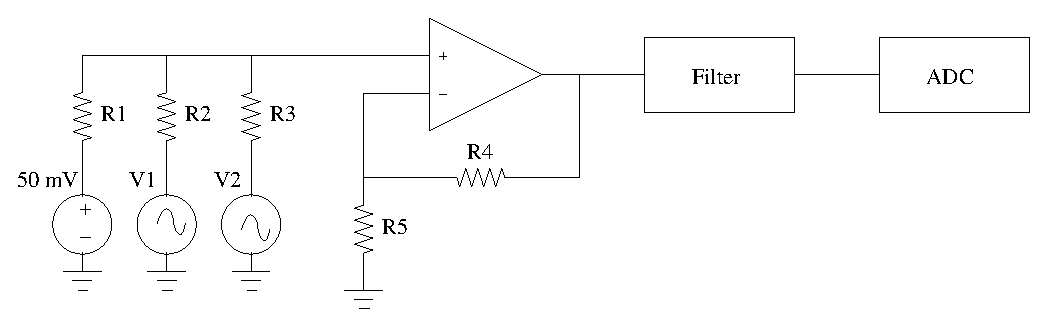
\includegraphics[width=0.75\linewidth]{sum_filt_adc.eps}\\

\emph{NOTE: The polarity of the op amp inputs are flipped compared to those in the first problem!!}

\begin{tabular}{cc}
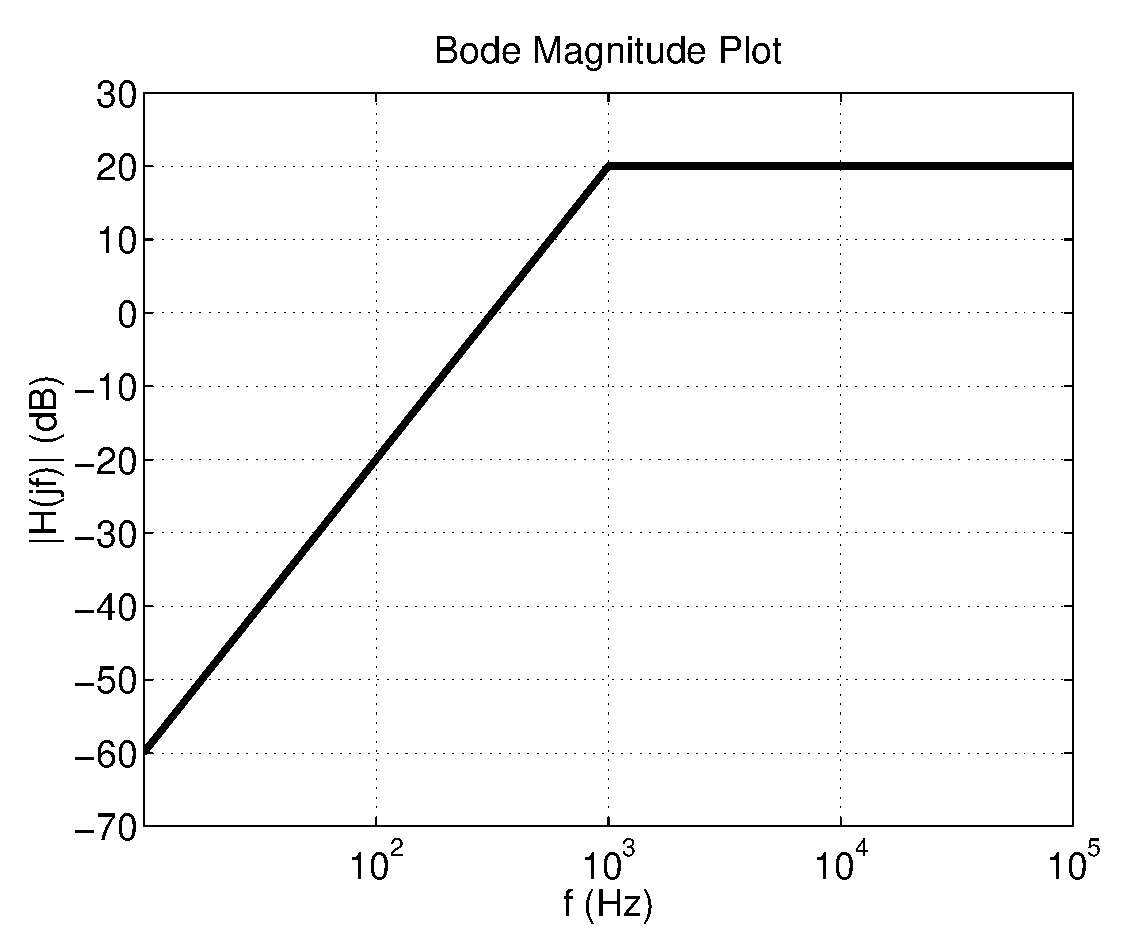
\includegraphics[width=0.4\linewidth]{bode_plot.eps} & 
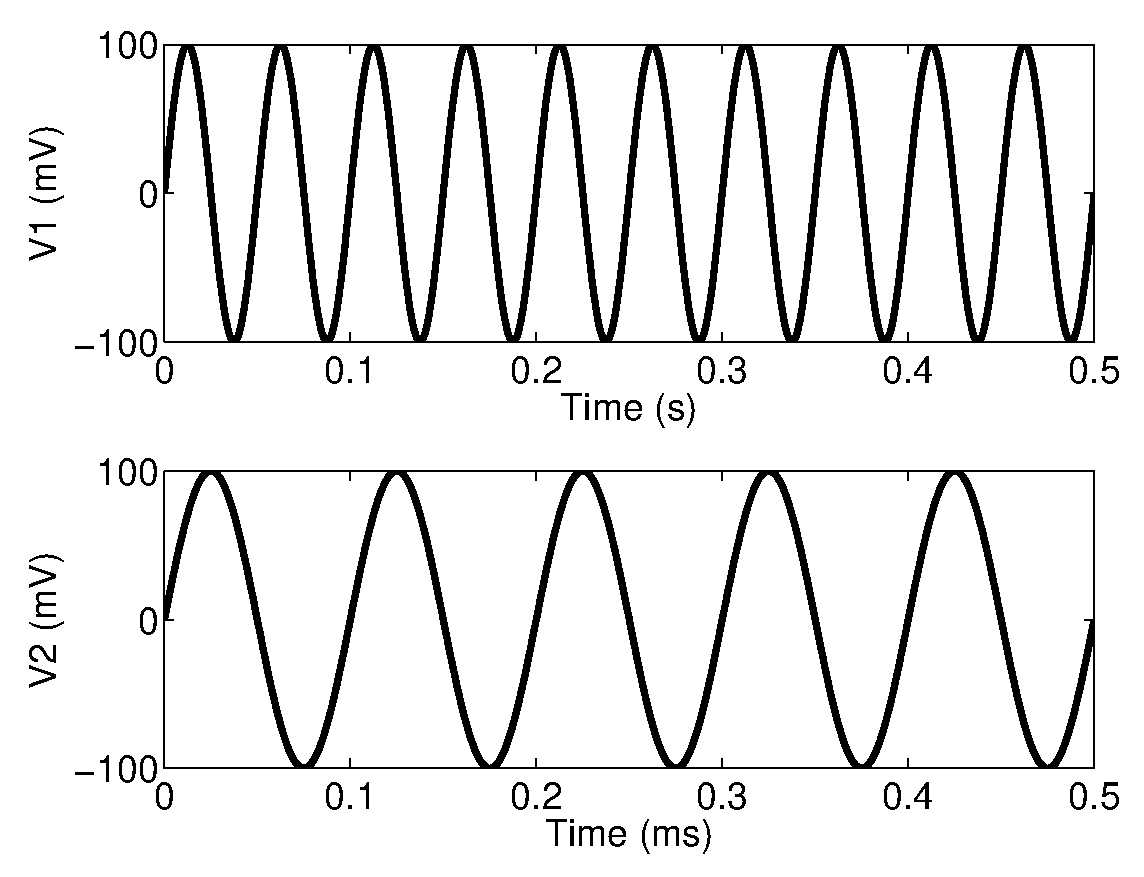
\includegraphics[width=0.4\linewidth]{sum_filt_adc_v1_v2.eps}\\
\end{tabular}


\end{center}

\begin{itemize}
\item $V_1$ and $V_2$ are continuous AC voltage sources with sample time waveforms shown in the plots above.
\item $R_1$ = $R_5$ = 5 k$\Omega$, $R_2$ = $R_3$ = $R_4$ = 10 k$\Omega$
\end{itemize}

\begin{enumerate}
\item Write an expression for the voltage output from the op amp before the
filtering stage.  (Don't worry about simplifying your answer too much.)
\item The op amp is setup to be what type of amplifier?  (Note - we did not directly cover this in class, but it is a variant of something that we did cover.)
\item The reason why we didn't cover this amplifier in class is because it has
a very bad input characteristic.  Solve for the input impedance as seen from
the 50 mV DC voltage source going ``into'' $R_1$.  Why is this ``bad''?
(Again, don't worry about simplifying your answer too much.)
\item Design a filter to achieve the characteristics shown in the Bode plot.
(Note that the phase characteristics of this filter have not been specified.)

\hfill{There is more on the next page...}
\clearpage

{\bf BME154L - Spring 2012 - Exam \#2 Solutions}\hfill Name (Net ID):\underline{\hspace*{3.0in}}



\item What is the voltage level associated with the least significant bit if
the ADC generates an 8-bit number that covers the full range of the signal from
the filter?  You do not need components of the input signal that are removed by
the attenuation band of the filter to be captured by the ADC (Don't worry about
an incorrect answer from an earlier part affecting your answer here; just
continue to solve these questions with the waveform that you have, which
hopefully is realistic.)
\item What is the ADC's theoretical minimum sampling frequency to accurately
capture the frequency content of the input signal?  In practice, what would be
a more reasonable minimum sampling frequency?
\item Compare/contrast the benefits/drawbacks of using a flash ADC versus a
successive approximation ADC.
\item Given your more realistic sampling frequency, if you had 16 kilobytes
(kB) of memory, how long could you continuously sample data from this circuit
before you would fill your memory register?
\end{enumerate}

\clearpage

{\bf BME154L - Spring 2012 - Exam \#2 Solutions}\hfill Name (Net ID):\underline{\hspace*{3.0in}}



\clearpage

{\bf BME154L - Spring 2012 - Exam \#2 Solutions}\hfill Name (Net ID):\underline{\hspace*{3.0in}}



\clearpage

{\bf BME154L - Spring 2012 - Exam \#2 Solutions}\hfill Name (Net ID):\underline{\hspace*{3.0in}}



\section{[35 points]}

Thermoelectric cooling relies on the Peltier effect to create a heat flux
between two different materials.  A Peltier device acts as a solid-state ``heat
pump'' that cools one material while heating the other.  You need to design a
Peltier device to cool a bioreactor to 15 $^\circ$C.  You want the cool side of
the Peltier device to stay near this temperature, but you can't run the device
if the hot side exceeds 30 $^\circ$C, otherwise you'll destroy the unit.  

You have 4 thermistors that you can use to monitor the cold and hot sides of
the Peltier device; these thermistors are identical and have a behavior
governed by the equation $\Delta R = k \Delta T$, where $k$ = 1 $\pm$ 0.02
$\Omega/^\circ C$ and $R$ = 10 k$\Omega$ at $T$ = 25 $^\circ$C.

When the Peltier device is ``on'', it requires 12 V DC and draws a current of 4
A; therefore, it needs to be electrically isolated from any transduction /
control circuitry.

Design a feedback circuit, similar to what you did in lab and the problem sets,
to (1) turn on the Peltier device when the cold side of the Peltier device is
$>$ 15 $^\circ$C, but (2) only when the hot side of the Peltier device is $<$
30 $^\circ$C.

There are lots of ways to do this!!  Show all of your work, including a block
diagram, and state all of your assumptions.  In addition to the thermistors
(you don't have to use all 4 if you don't want to), you can use whatever
resistors, power sources, op amps, capacitors, inductors, logic gates, etc.
that you would like in your circuit.  Full credit will be awarded for circuit
designs that maximize SNR and minimize the number of circuit components needed
to achieve the functional goals.

\clearpage

{\bf BME154L - Spring 2012 - Exam \#2 Solutions}\hfill Name (Net ID):\underline{\hspace*{3.0in}}



\clearpage

{\bf BME154L - Spring 2012 - Exam \#2 Solutions}\hfill Name (Net ID):\underline{\hspace*{3.0in}}



\end{document}
